\documentclass{beamer}
\usetheme{Madrid}
\usecolortheme{spruce}

% Number captions
\setbeamertemplate{caption}[numbered]

% Number bibliography entries
\setbeamertemplate{bibliography item}{\insertbiblabel}

% Change base colour beamer@blendedblue (originally RGB: 0.2,0.2,0.7)
\colorlet{beamer@blendedblue}{green!40!black}

\usepackage{lmodern}
\usepackage{caption}

\usepackage[citestyle=authoryear, sorting=none]{biblatex}
\addbibresource{databall.bib}
\DeclareNameAlias{sortname}{last-first}
\DeclareNameAlias{default}{last-first}

\title{DataBall}
\subtitle{Predicting NBA Winners with Data}
\author{Kevin Lane}

\begin{document}

\begin{frame}
\titlepage
\end{frame}

\begin{frame}
\frametitle{Outline}
\tableofcontents
\end{frame}

\section{Introduction}

\subsection{Background}
\begin{frame}
\frametitle{Background}
\begin{itemize}
    \item Sports analytics began in professional baseball, most notably with the work of Bill James\footcite{james}
    \begin{itemize}
        \item James coined the term sabermetrics as ``the search for objective knowledge about baseball''
        \item James selected the name to honor the Society for American Baseball Research (SABR)
    \end{itemize}
    \item Gained widespread adoption after Billy Beane implemented James' ideas and led the Oakland Athletics to a record winning streak\footcite{lewis}
    \item Analytics has since spread to other sports and its impact is evidenced by several examples:
    \begin{itemize}
        \item MLB's increased attention to on-base percentage beginning in the Moneyball era of the early 2000s
        \item The rise of the three-point shot and subsequent fall of the midrange jumper in the NBA
        \item Increased use of short, high percentage passes in the NFL
    \end{itemize}
\end{itemize}
\end{frame}

\begin{frame}
\frametitle{Background}
\begin{block}{What makes sports an attractive testbed for machine learning?}
According to Nate Silver, ``sports nerds have it easy.''\footnotemark
\begin{enumerate}
    \item ``Sports has awesome data.''
    \item ``In sports, we know the rules.''
    \item ``Sports offers fast feedback and clear marks of success.''
\end{enumerate}
\end{block}
\footcitetext{silver-online}
\vspace{-0.5cm}
\begin{block}{Why the NBA?}
\begin{itemize}
    \item Easily the most deterministic of the major American sports
    \item The NBA provides a wealth of advanced stats and player tracking data on their website
    \item The season is long enough at 82 games that sample size is not as much of a concern as in the NFL, who claim to have parity, but also only play 16 regular season games
\end{itemize}
\end{block}
\end{frame}

\subsection{Process}
\begin{frame}
\frametitle{Process}
\begin{itemize}
    \item I used several algorithms from the popular Python machine learning library scikit-learn\footcite{scikit-learn} to predict NBA game winners
    \begin{itemize}
        \item Logistic Regression
        \item Support Vector Machine
        \item Random Forest
        \item Multilayer Perceptron
        \item Na{\"i}ve Bayes
    \end{itemize}
    \item I used box score data from the 1990-91 season through 2015-16
    \item The games are split into training and test sets randomly, so games from future seasons are used to predict past games
    \begin{itemize}
        \item This does not provide a realistic scenario for making predictions in real time, such as in betting
        \item Provides a easy way to compare several algorithms and feature combinations, which will help inform future work
    \end{itemize}
    \item All models are trained with season-averaged team stats
\end{itemize}
\end{frame}

\section{Data}

\subsection{Data Wrangling}
\begin{frame}
\frametitle{Data Wrangling}
\begin{itemize}
    \item I collected stats from the NBA's stats website \url{stats.nba.com}
    \begin{itemize}
        \item The site exposes a wealth of information in JSON format through various web API endpoints
        \item I utilized the GitHub project nba\_py to format the URLs and collect stats into Pandas DataFrames
    \end{itemize}
    \item I stored all collected stats to a SQLite database using Python's built-in SQLite support
    \item I used the basic box score stats to calculate more advanced stats
    \begin{itemize}
        \item Offensive/defensive ratings (points scored/allowed per 100 possessions), which requires an estimate for the number of possessions
        \item Simple Rating System (SRS), which is a team's average margin of victory adjusted for its strength of schedule
        \item Oliver's four factors\footcite{oliver}, which include effective FG\%, TOV\%, OREB\%, and free throw rate
        \item Weighted four factors, which is just sum of the four factors weighted according to Oliver's assigned weights
    \end{itemize}
\end{itemize}
\end{frame}

\subsection{Data Exploration}
\begin{frame}
\frametitle{Data Exploration}
\begin{columns}
\column{0.5\textwidth}
\begin{itemize}
    \item The top figure shows that the home team winning percentage is remarkably consistent
    \begin{itemize}
        \item Simply predicting the home team wins will yield about 60\% accuracy
        \item This provides a good baseline; any predictive model worth implementing should beat this
    \end{itemize}
    \item The bottom figure shows that team performance (according to SRS) very closely resembles a normal distribution
    \begin{itemize}
        \item An SRS of zero indicates an average team
    \end{itemize}
\end{itemize}
\column{0.5\textwidth}
\vspace{-0.5cm}
\begin{figure}
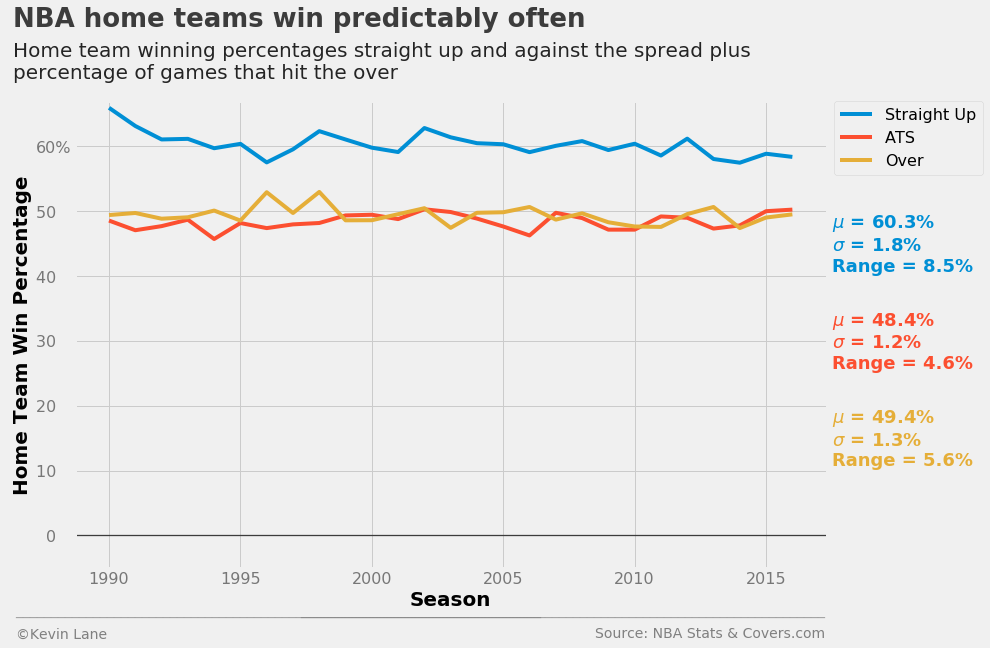
\includegraphics[width=60mm]{../docs/assets/images/data-exploration/home-win-pct.png}
\end{figure}
\vspace{-0.5cm}
\begin{figure}
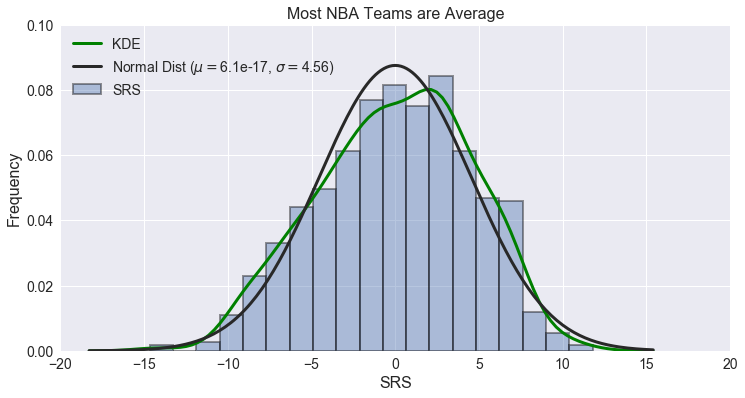
\includegraphics[width=60mm]{../docs/assets/images/data-exploration/srs-distribution.png}
\end{figure}
\end{columns}
\end{frame}

\begin{frame}
\frametitle{Data Exploration}
\begin{itemize}
    \item The plots below show kernel density estimations (KDE) of SRS split between home team wins and losses
    \item The dark region to the bottom right of the origin for home team wins shows above-average home teams tend to beat below-average visitors
    \item The opposite appears in the KDE of home team losses
\end{itemize}
\begin{figure}
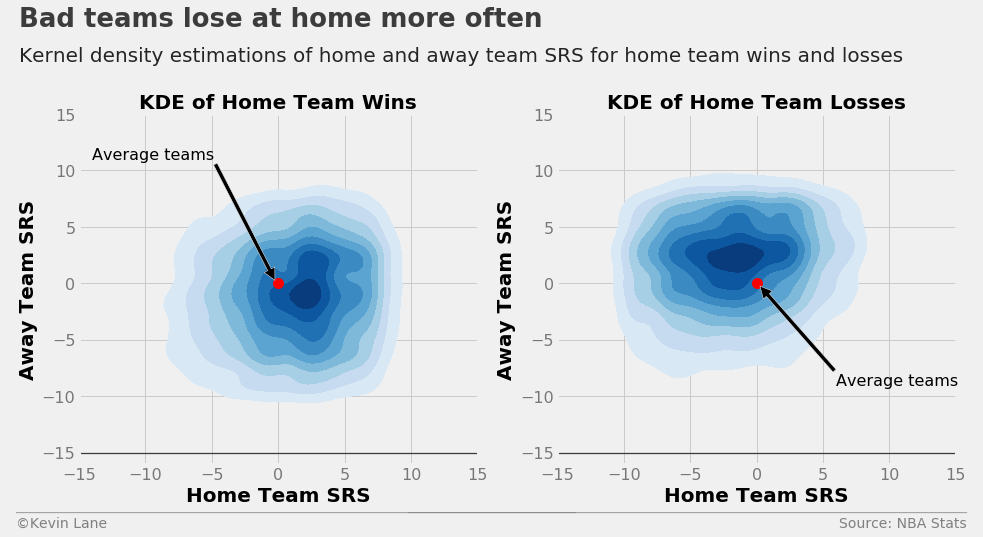
\includegraphics[scale=0.35]{../docs/assets/images/data-exploration/srs-win-loss-kde.png}
\end{figure}
\end{frame}

\section{Model Selection}

\subsection{Feature Selection}
\begin{frame}
\frametitle{Feature Selection}
\begin{itemize}
    \item The plots below show cross-validation ROC and precision/recall curves using home and away SRS
    \item The folds show little spread, so we are confident the cross-validation results in a good estimate of model performance
\end{itemize}
\begin{figure}
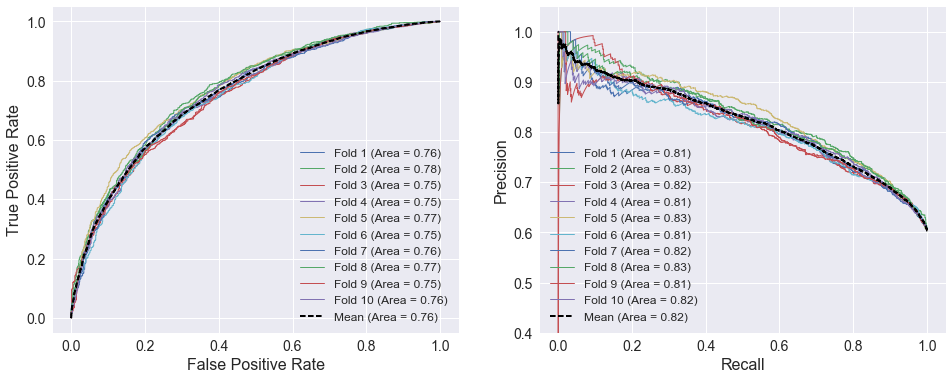
\includegraphics[scale=0.35]{../docs/assets/images/feature-selection/srs-cross-validation.png}
\end{figure}
\end{frame}

\begin{frame}
\frametitle{Feature Selection}
\begin{itemize}
    \item The plots below show cross-validation ROC and precision/recall curves for various metrics
    \item All point-related metrics (SRS, Plus/Minus, etc.) are nearly identical
    \item The point-related metrics outperform the two metrics based on the four factors
\end{itemize}
\begin{figure}
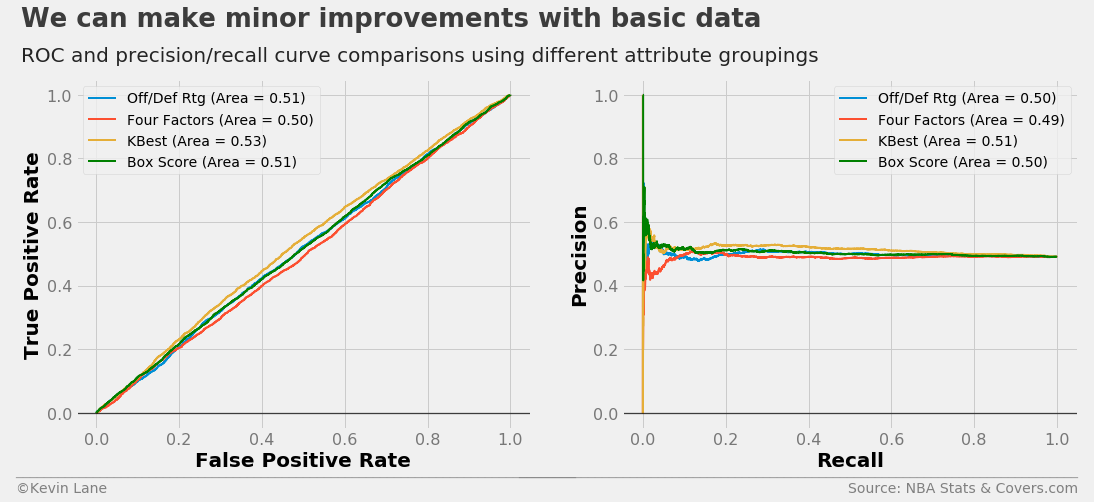
\includegraphics[scale=0.35]{../docs/assets/images/feature-selection/cross-validation-comparison.png}
\end{figure}
\end{frame}

\subsection{Parameter Tuning}
\begin{frame}
\frametitle{Parameter Tuning}
\begin{itemize}
    \item Parameter tuning did not yield models that performed noticeably better than the default models
\end{itemize}
\begin{figure}
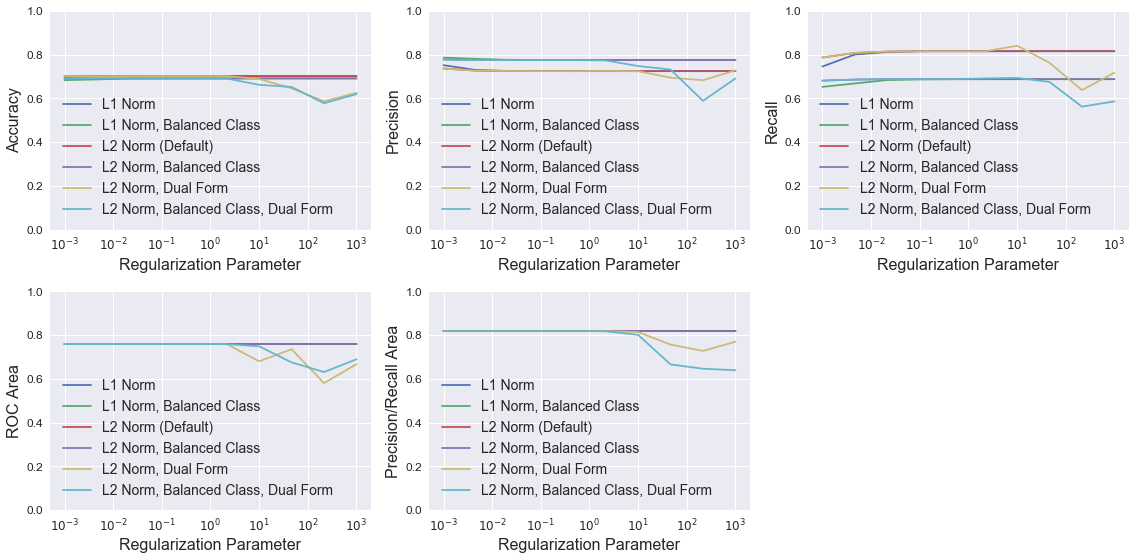
\includegraphics[scale=0.3]{../docs/assets/images/parameter-tuning/logistic-regression-metrics.png}
\caption{Logistic Regression Parameter Tuning}
\end{figure}
\end{frame}

\section{Results}

\subsection{Model Performance}
\begin{frame}
\frametitle{Model Performance}
\begin{columns}
\column{0.5\textwidth}
\begin{itemize}
    \item Logistic regression does a great job at predicting home wins (81.5\% accuracy), but struggles with home losses (about 50\% accuracy)
    \item These general numbers hold true for all the models tested except the random forest model, which performed about 10\% worse predicting home wins
    \item Additional effort should be focused on improving home loss predictions to improve overall model performance
    \begin{itemize}
        \item One option is to down sample home wins to achieve a 50/50 split of the two classes
    \end{itemize}
\end{itemize}
\column{0.5\textwidth}
\vspace{-0.5cm}
\begin{figure}
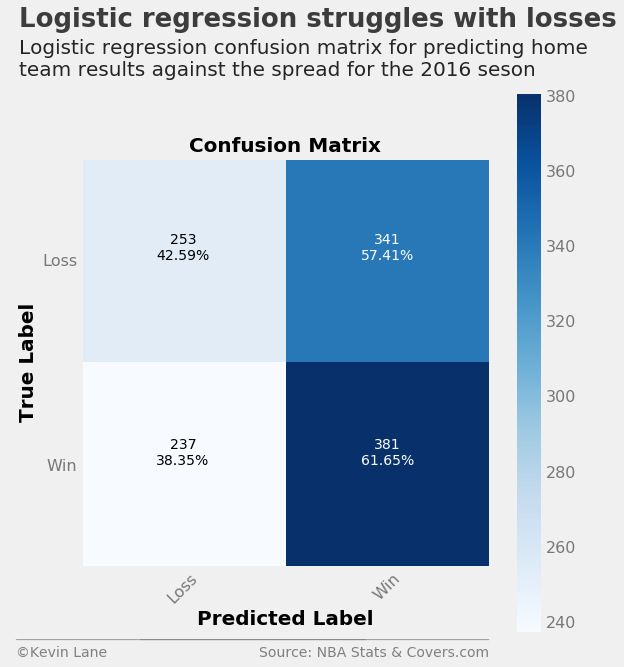
\includegraphics[scale=0.23]{../docs/assets/images/model-performance/logistic-regression-confusion-matrix.png}
\caption{Logistic Regression CM}
\end{figure}
\vspace{-1cm}
\begin{figure}
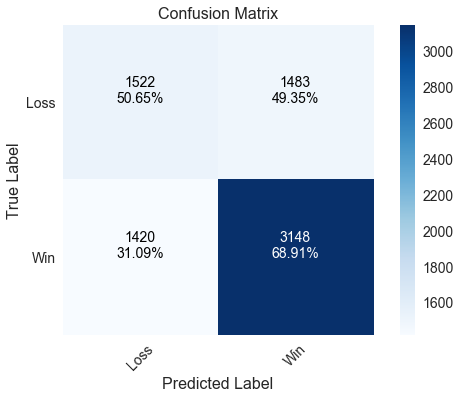
\includegraphics[scale=0.23]{../docs/assets/images/model-performance/random-forest-confusion-matrix.png}
\caption{Random Forest CM}
\end{figure}
\end{columns}
\end{frame}

\begin{frame}
\frametitle{Model Performance}
\begin{itemize}
    \item All models performed about the same with the exception of the random forest model
    \item The random forest performed about the same with home losses, but had degraded performance predicting home wins
\end{itemize}
\begin{figure}
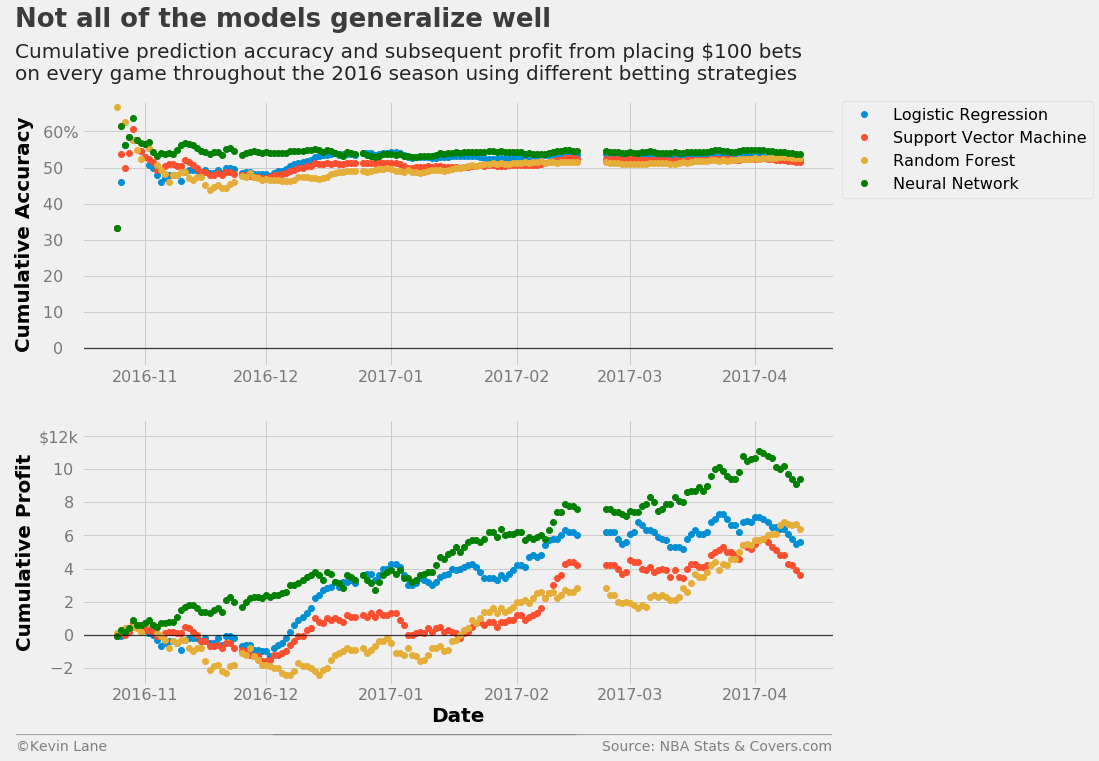
\includegraphics[scale=0.35]{../docs/assets/images/model-performance/model-performance-comparison.png}
\caption{Model Performance Comparison}
\end{figure}
\end{frame}

\subsection{Comparison to Published Results}
\begin{frame}
\frametitle{Comparison to Published Results}
\begin{itemize}
    \item The roughly 70\% prediction accuracy is in line with published results
    \item Zimmermann\footcite{zimmermann} used algorithms in Weka\footcite{witten} to predict NBA and NCAA game winners
    \begin{itemize}
        \item He trained the models using data from previous games, making it a more realistic scenario
        \item He correctly predicted about 57-68\% of NBA games correctly, though most seasons were below 64\% accuracy
        \item He was much more successful in the NCAA, where the range in skill level is much larger than the NBA
    \end{itemize}
    \item Loeffelholz et al.\footcite{loeffelholz} used the MATLAB neural network toolbox to predict NBA game winners
    \begin{itemize}
        \item They performed a cross-validation similar to what was shown here
        \item They only examined part of one season (only 30 games used for testing)
        \item They predicted approximately 74\% of games correctly, but it is unclear if this generalizes well
    \end{itemize}
\end{itemize}
\end{frame}

\section{Future Work}

\begin{frame}[t]
\frametitle{Future Work}
\begin{itemize}
    \item Train models with prior games to permit ``real time'' predictions and update the models as each season progresses
    \item Incorporate player stats to adjust predictions as rosters fluctuate
    \item Predict winners against Vegas spreads
    \begin{itemize}
        \item Track return on investment (ROI) if a prospective bettor were to bet on the model's predicted winners
        \item Incorporate a confidence threshold to investigate how ROI changes when bets are only made on games in which the model's confidence exceeds the threshold
    \end{itemize}
\end{itemize}
\end{frame}

\section{References}

\begin{frame}[t, allowframebreaks]
\frametitle{References}
\printbibliography
\end{frame}

\end{document}
